\chapter{双模式检查点生成技术及混合内存性能优化}
\label{chap:thnvm}

\section{软件透明的一致性保证机制}

新兴的字节编址的(byte-addressable)非易失性内存介质,诸如STT-RAM~\cite{4443191}、PCM~\cite{Raoux:2008:PRA}和ReRAM~\cite{5607274}等预示着持久化内存系统,一个在内存和存储栈上的新的中间层。持久化内存系统融合了传统内存系统(快速的load/store指令接口)和存储系统(数据持久化)的优良特性,模糊了两者之间的界限。它给应用带来的一个重要的益处是,可以通过load/store指令高效地直接地访问内存中的持久化数据,而不需要与存储设备进出换页、在(反)序列化时更改数据格式以及触发臃肿的系统调用。

持久化内存相对于传统的易失性内存系统引入了一个关键的要求,系统故障时的一致性保证~\cite{Lamb:1991:ODS,Copeland:1989:CSR,Shapiro:1999:EFC}。这要求持久化内存系统,在掉电或系统失效等故障出现时,依然能够保证数据的一致性不受部分或是乱序的NVM写的影响。我们以原子性地更新保存在NVM上的数据结构A和B为例,总会有对A或B的一个更改会先于其他写入NVM。如果系统在一个更改完成之后出现故障或掉电,两个数据结构可能处于不一致的中间状态,只包含部分更改。对于传统易失性内存,这不是一个问题,因为程序恢复后内存中的数据都会丢失。但对于持久化内存,这些不一致的数据会一直保留。所以,持久化内存系统需要保证保存到NVM的数据可以在系统重启后恢复到一个一致的状态,即维持数据的一致性。维持数据的一致性原本仅是对磁盘或闪存等存储系统的要求,但将数据持久化引入内存后,它即成为内存系统同样面临的一个挑战。

大多数之前的持久化内存设计依赖于程序员的人工努力来保证系统故障时的数据一致性。应用的开发人员需要显式地使用特定的编程模型和软件接口来访问和操作内存中的持久化数据。这些软件接口构建于为持久化内存定制的运行时库~\cite{Condit:2009:BIT:1629575.1629589,Volos:2011:MLP:1950365.1950379}或硬件架构~\cite{Zhao:2013:KCP:2540708.2540744}。这种设计似乎给程序员提供了对数据持久化的完全控制,但要求程序员管理持久化内存会带来至少三方面不良影响。首先,应用开发者必须用新的编程接口API来实现程序或者深度更改遗留代码,通常要显式地声明和划分持久的和临时数据结构。其次,大多数之前的持久化内存设计需要使用事务性内存控制版本和对NVM写的顺序,而事务性内存的扩展性依然面临挑战。第三,现在持久性内存的编程模型可能基于很多种语义和软件接口实现,会带来兼容性和移植性问题。为此,我们工作的目标是设计高效的故障时数据一致性保障机制,使得持久化内存的使用范围得到扩展而不必需要复杂的应用更改。

我们提出了THNVM,一种新的支持对软件透明的故障时数据一致性的持久化内存设计。它允许基于事务的和基于锁的程序直接在持久化内存硬件上运行。THNVM使用DRAM和NVM混合的架构和高效的硬件辅助的检查点生成技术来达到DRAM水平的性能。这里的一个关键挑战是减少由于生成检查点而导致的应用停滞时间。我们发现,在停滞时间和元数据存储开销之间存在一个折衷。在较小的粒度上生成检查点,带来的停滞时间可以比较短,而对应元数据占用的空间却会非常大;在较大的粒度上生成检查点,可以降低元数据占用的空间,但是会导致较长的停滞时间。因此,单一的检查点生成技术(或者基于小粒度或者基于大粒度)难以达到最优的效果。为了解决这一问题,我们提出了双模式检查点生成机制,它可以同步地为分散的和集中的内存写分别基于CPU缓存块粒度和操作系统页粒度生成检查点。与先前使用写时拷贝(copy-on-write,COW)或日志技术的持久化内存设计相比,THNVM显著减小了存储的损耗并增加了内存带宽的利用率。

特别地,本章工作做出了如下几点贡献:(1)我们提出了一种新的持久化内存设计,支持对软件透明的故障时数据一致性保障。我们的设计允许基于事务的和基于锁的应用通过load/store指令接口使用持久化内存。(2)对于生成检查点的粒度,我们定位了程序停滞时间和元数据空间占用之间的权衡关系。在任意一个粒度上追踪对持久化内存的更改都不是最优的。(3)我们设计了一个新的双模式检查点生成技术。我们的技术比页粒度的检查点生成机制减少了86.2\%的停滞时间,而仅比缓存块粒度的检查点生成机制多用26\%的内存控制器硬件空间。(4)我们在内存模拟器上实现了双模式检查点生成机制,使用我们经过形式化证明的一致性协议。它可以在保证数据一致性的同时,将检查点生成过程和程序执行重叠。我们的解决方案可以达到不提供一致性支持的全DRAM系统性能的95.1\%。

\section{现有技术缺陷}

THNVM的设计有三个本质特性:软件透明,检查点生成,以及双模式。本节讨论我们开发这三种特性的原因。

\subsection{软件一致性保障技术的缺陷}

\begin{figure}[t]
\centering 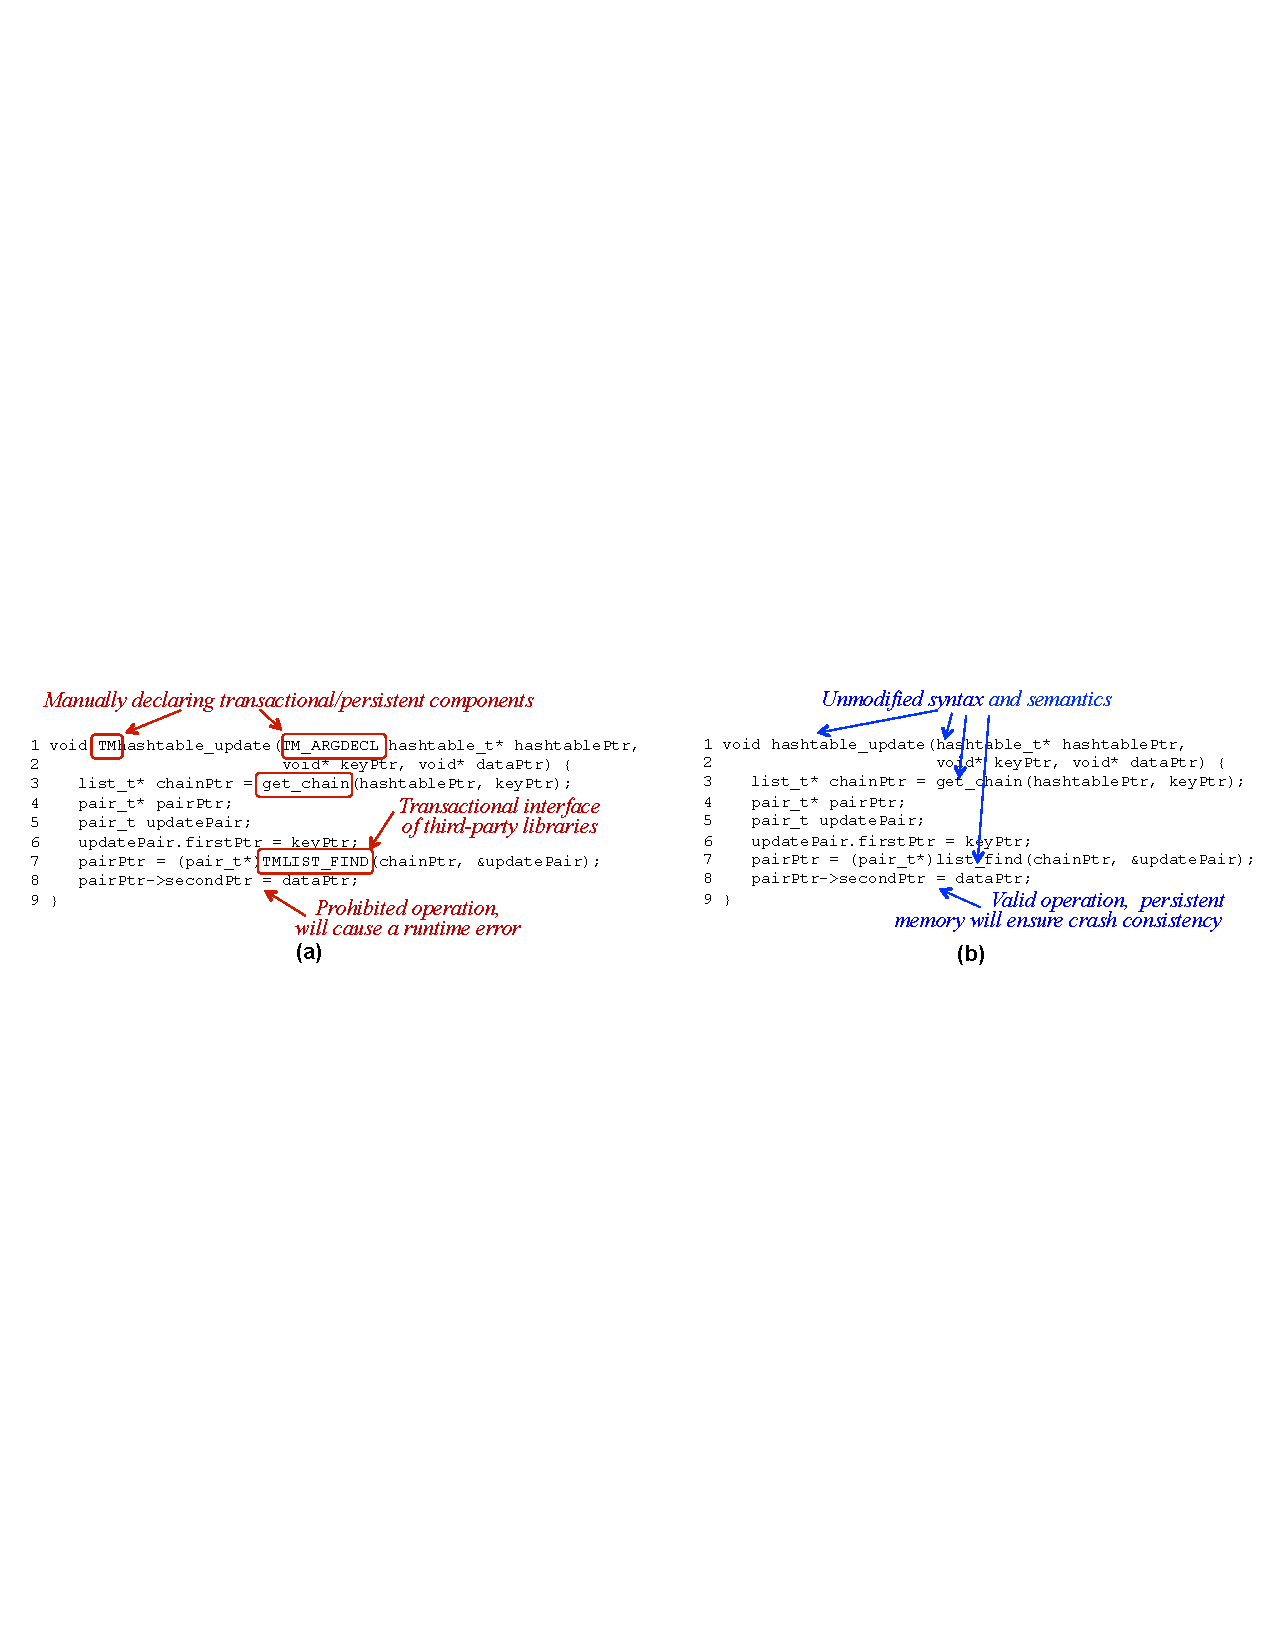
\includegraphics[width=\columnwidth]{motivation-code}
  \caption{实例代码:向持久化的哈希表中插入一个项。分别采用(a)传统的软件接口或(b)软件透明的THNVM。}
\label{fig:motivation-code}
\end{figure}

之前大多数持久化内存设计~\cite{Condit:2009:BIT:1629575.1629589,Volos:2011:MLP:1950365.1950379,Coburn:2011:NMP:1950365.1950380,Zhao:2013:KCP:2540708.2540744,Venkataraman:2011:CDD:1960475.1960480}要求应用开发者显式地定义持久性数据并使用特定库来访问数据——故障时数据一致性保障机制与软件的语义紧耦合。我们通过图\ref{fig:motivation-code}中的实例代码来展示这种持久化内存设计的不足。该图比较了一个更新持久性哈希表项的软件方法的两种实现(代码改编自STAMP~\cite{Cao:2008:STA})。图\ref{fig:motivation-code}(a)展示了使用类似于现有设计~\cite{Condit:2009:BIT:1629575.1629589, Volos:2011:MLP:1950365.1950379}的软件事务的实现;而图\ref{fig:motivation-code}(b)中的实例代码采用了THNVM的软件透明的故障时数据一致性支持。我们可以看到,在支持数据一致性时涉及软件支持,会有多方面的不足。

首先,划分临时性和持久性数据很麻烦而且容易出错。图\ref{fig:motivation-code}(a)展示了许多无法避免的标记。程序员需要对软件行为有深入的了解,并且小心地确定哪些数据结构需要持久化以及如何操控这些数据。例如,图\ref{fig:motivation-code}(a)的第3行仅当这个哈希表实现固定数目的桶时才是正确的。

其次,在一个统一的地址空间内,临时性和持久性数据之间的引用需要小心的管理。然而,对该问题的基于软件的解决方案并非最佳。例如,为了处理NV-to-V指针(非易失性指针指向易失性数据,图\ref{fig:motivation-code}(a)的第8行),NV-heaps~\cite{Coburn:2011:NMP:1950365.1950380}会简单地抛出一个运行时错误以禁用此类指针。

第三,应用需要使用事务,通常是通过事务性内存接口(例如被Mnemosyne~\cite{Volos:2011:MLP:1950365.1950379}使用的TinySTM~\cite{Felber:2008:DPT}),来更新持久化数据,如图\ref{fig:motivation-code}(a)所示。遗憾的是,事务性内存,不论基于硬件还是基于软件,存在多方面的可扩展性问题~\cite{Cascaval:2008:STM:1454456.1454466,Pankratius:2011:STM:1989493.1989500,Dice:2009:EEC:1508244.1508263}。此外,开发人员必须使用新的API来实现或者重写各种代码库和程序,需要不可忽略的人工投入。不熟悉这些新API的程序员需要一个痛苦的学习过程。

最后,应用需要构建在特定的库之上,例如libmnemosyne~\cite{Volos:2011:MLP:1950365.1950379}和
NV-heaps~\cite{Coburn:2011:NMP:1950365.1950380}。这会很大程度上降低持久化内存应用的移植性——在一个库上实现的应用,如果想采用其他的库,需要重新实现。编译器确实可以在一定程度上减轻程序员实现和移植代码的负担。然而,编译器会无差别地插装所有内存的读和写操作,带来可见的性能损耗。我们在GCC libitm~\cite{libitm}上实验了STAMP事务性基准测试~\cite{Cao:2008:STA},结果插装本身最多可带来高达8\%的性能损失。

我们采用了允许软件程序直接访问持久化内存的使用模型。如图\ref{fig:motivation-code}(b)所示,我们可以不更改代码而实现数据结构的持久化。

\subsection{日志及写时拷贝技术的缺陷}

前人基于软件的持久化内存设计,大部分通过修改现有软件事务性内存库、文件系统或者数据库实现,采用日志~\cite{Volos:2011:MLP:1950365.1950379, Coburn:2011:NMP:1950365.1950380}或者写时拷贝技术~\cite{Condit:2009:BIT:1629575.1629589,
Venkataraman:2011:CDD:1960475.1960480}维持数据一致性。然而,两种技术为支持数据一致性保障会引入较大的性能损耗。

日志可能消耗比原始数据大很多的NVM空间,因为每个日志项都是一个既包含数据又包含元数据(例如数据所在的地址)的元组,而且通常每次写操作都需要记录~\cite{Volos:2011:MLP:1950365.1950379,
Coburn:2011:NMP:1950365.1950380}\footnote{某些对于日志的改进或变形~\cite{1003568}使用一个索引结构来合并更新。该设计即与我们双模式之一类似。}。此外,日志重放增加了故障后系统恢复时间,会抵消使用NVM而不是顺序访问的块设备带来的快速数据恢复的好处。

写时数据拷贝有两个缺点。首先,拷贝操作代价较大,会引发较长的停滞时间。其次,它不可避免地会复制未更改的数据,消耗额外的NVM带宽。这个缺陷在更新的地址很分散时尤为突出。

相比之下,生成检查点是一种更加灵活的方法,它定期地将易失性的数据及元数据写入NVM形成一致的内存数据的快照。我们仔细挑选和协调两种检查点生成模式,使它们同步地在不同粒度上工作,从而避免日志和写时拷贝的弊端。

\subsection{粒度的权衡}

CPU缓存在块粒度上(典型配置为64字节)管理数据;操作系统在页粒度上(典型配置为4KB)管理数据。我们发现两个不同的粒度会带来一个在检查点生成停滞时间和元数据存储空间之间的折衷。

当我们选择在缓存块粒度上追踪持久化内存的更改时,各个细粒度写如果直接发送到NVM,可以在一两次总线传输的延迟内完成。这样,THNVM只需要在生成检查点时将追踪这些数据所用的元数据进行持久化即可。这些元数据可以保存在一个表中,每个表项保存一个从缓存块在内存中的地址到它实际检查点或工作数据位置的映射。这种模式的缺点在于元数据表项的数量是按页粒度追踪数据所需表项的64倍,因为每个页包含64个缓存块。相反地,如果我们在页粒度上追踪持久化内存的更改,我们可以极大地降低保存元数据表所需的硬件空间开销。然而把整页的数据写入NVM所造成的延迟,远大于更新一个缓存块。为了提升系统性能,THNVM使用DRAM来缓冲页粒度的更新,一段时间后再在NVM上生成这些页的检查点。尽管如此,将整页数据从DRAM传送到NVM依然会给系统带来较长的停滞时间。

考虑到如上的折衷,只在一个粒度上追踪持久化内存的更改不是最佳方案。这种情况下,我们需要开发一种双粒度的检查点生成技术。

\section{双模式检查点生成技术}

\begin{figure}[t]
\centering
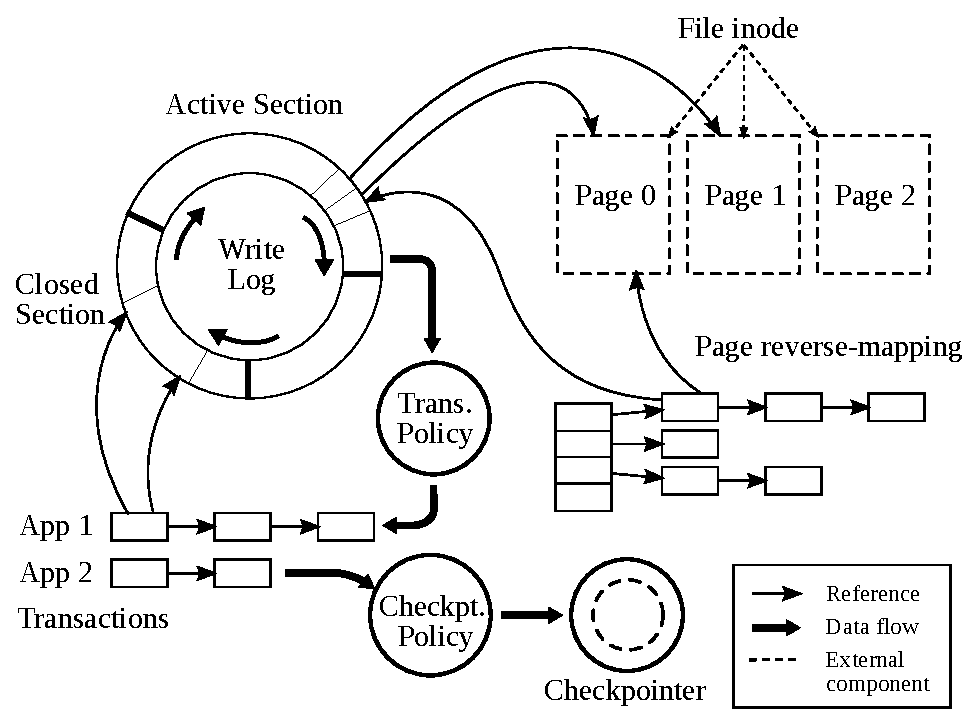
\includegraphics[width=0.8\columnwidth]{arch}
\caption{THNVM的总体架构图}
\label{fig-arch}
\end{figure}

THNVM采用DRAM和NVM的混合架构,基于硬件实现,提供软件透明的故障时数据一致性保障。THNVM以透明于应用程序的方式保障所有内存数据在故障时的一致性。为了利用在不同粒度持久化数据带来的不同特性,我们提出了一种新的双模式检查点生成机制。它可以同时在两个粒度上生成内存数据的检查点:分散的写在缓存块粒度上生成检查点,使用块重映射模式(第\ref{subsec:block-remap}节);集中的写在页粒度上生成检查点,使用页回写模式(第\ref{subsec:page-writeback}节)。

另外,我们提出了两种机制来协调双模式检查点生成(第\ref{subsec:coordination}节)。第一,我们允许相对较快的块重映射模式来暂时接管原本应该由较慢的页回写模式处理的写。这样做可以显著减少检查点生成阻塞程序执行的时间。第二,我们定期地依据程序执行时访问内存的特点在两种模式之间迁移数据页。这样做可以有效保证检查点生成模式和其处理的写的行为相匹配。

图\ref{fig-arch}绘制了THNVM架构总览。DRAM和NVM部署在内存总线上,并映射到同一个物理内存地址空间中。该地址空间暴露给操作系统。我们更改了内存控制器,增加了一个检查点生成控制器,和两个用于维护内存访问元数据的地址转换表。这两个表分别是在缓存块粒度和页粒度管理元数据的块转换表(block translation table,BTT)和页转换表(page translation table,PTT)。

\subsection{系统定义}

\textbf{失效模型}:THNVM允许软件应用在诸如系统死机、掉电等故障发生后,从一个一致的内存数据检查点开始,继续CPU执行。为此,我们需要定期将内存中的数据的更新和CPU状态生成检查点,这其中包括CPU寄存器、写缓冲、脏缓存块以及内存控制器的写队列。我们的检查点生成机制保护内存数据和CPU状态的一致性不因系统故障而被污染。

\begin{figure}[t]
\centering
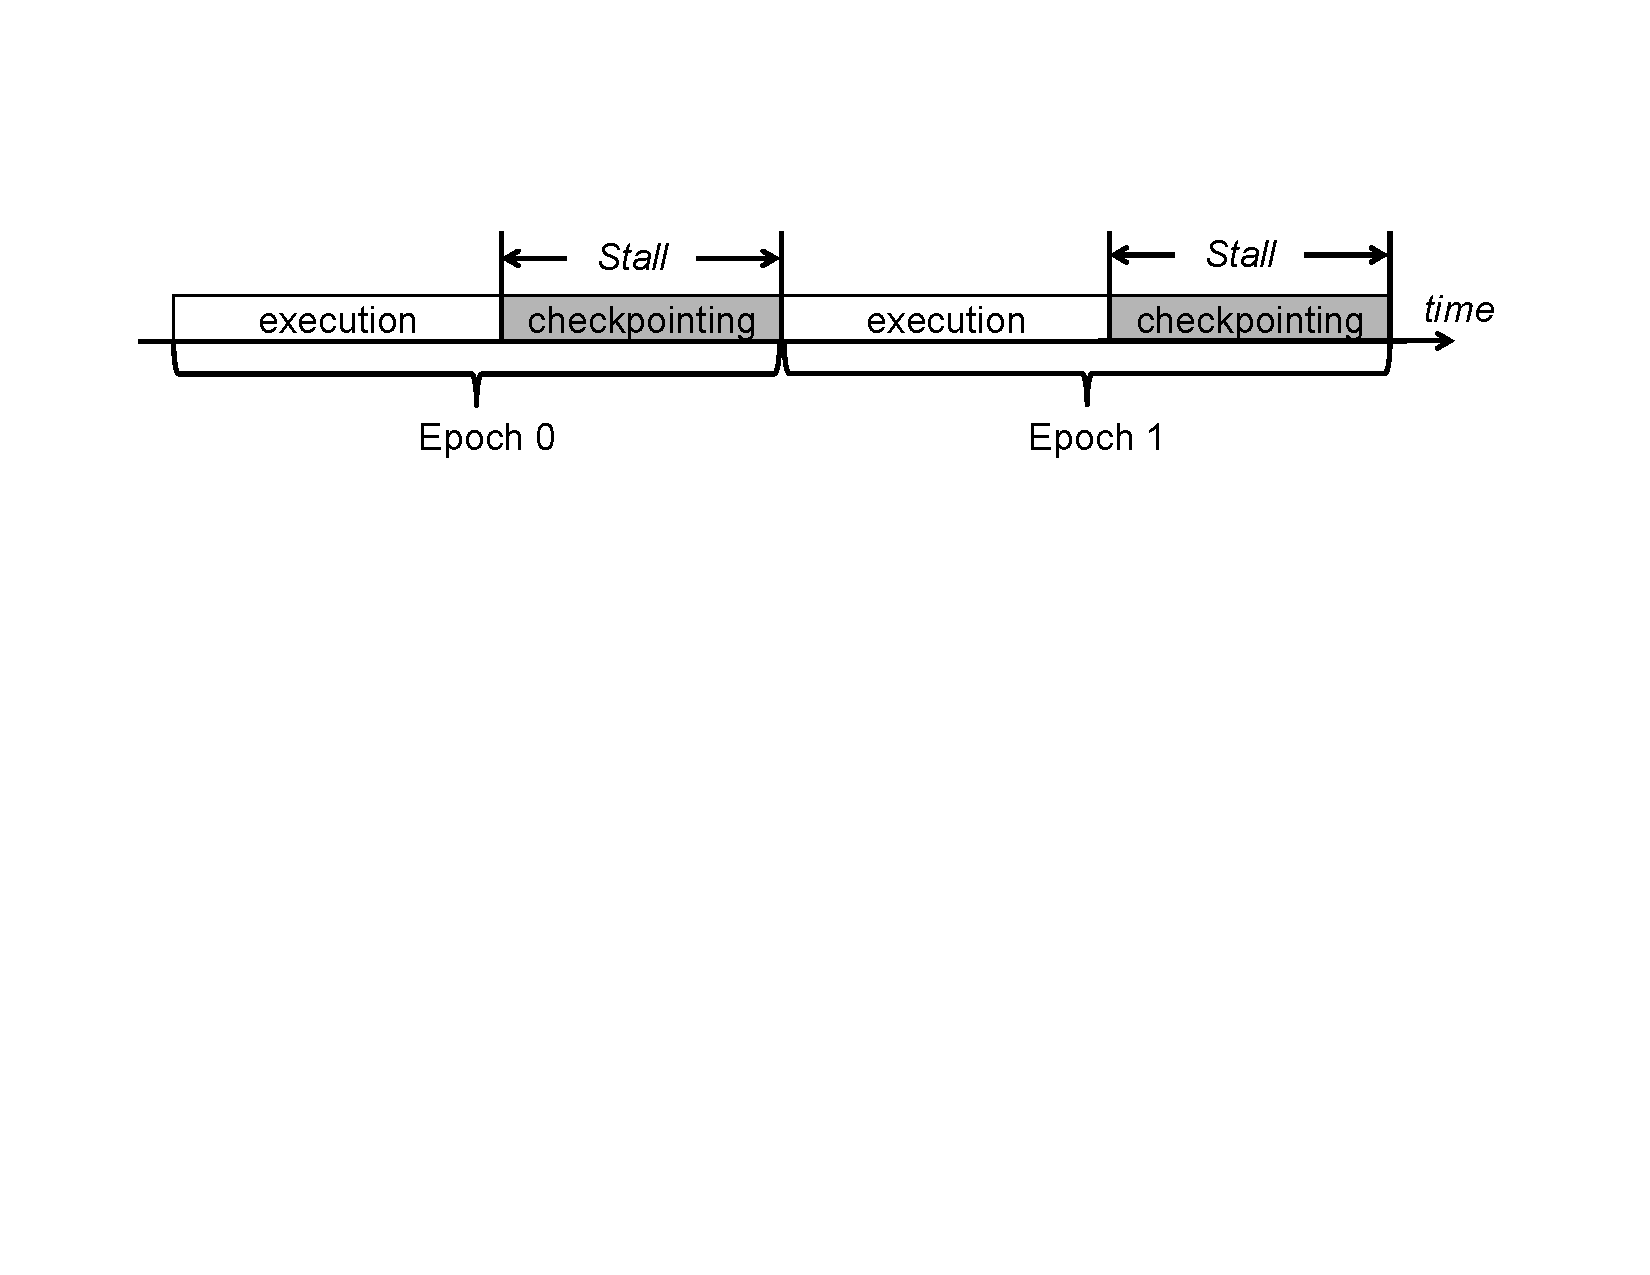
\includegraphics[width=0.9\columnwidth]{epoch-before}\\
{\small (a) 采用检查点生成时暂停全系统的时间单元模型}
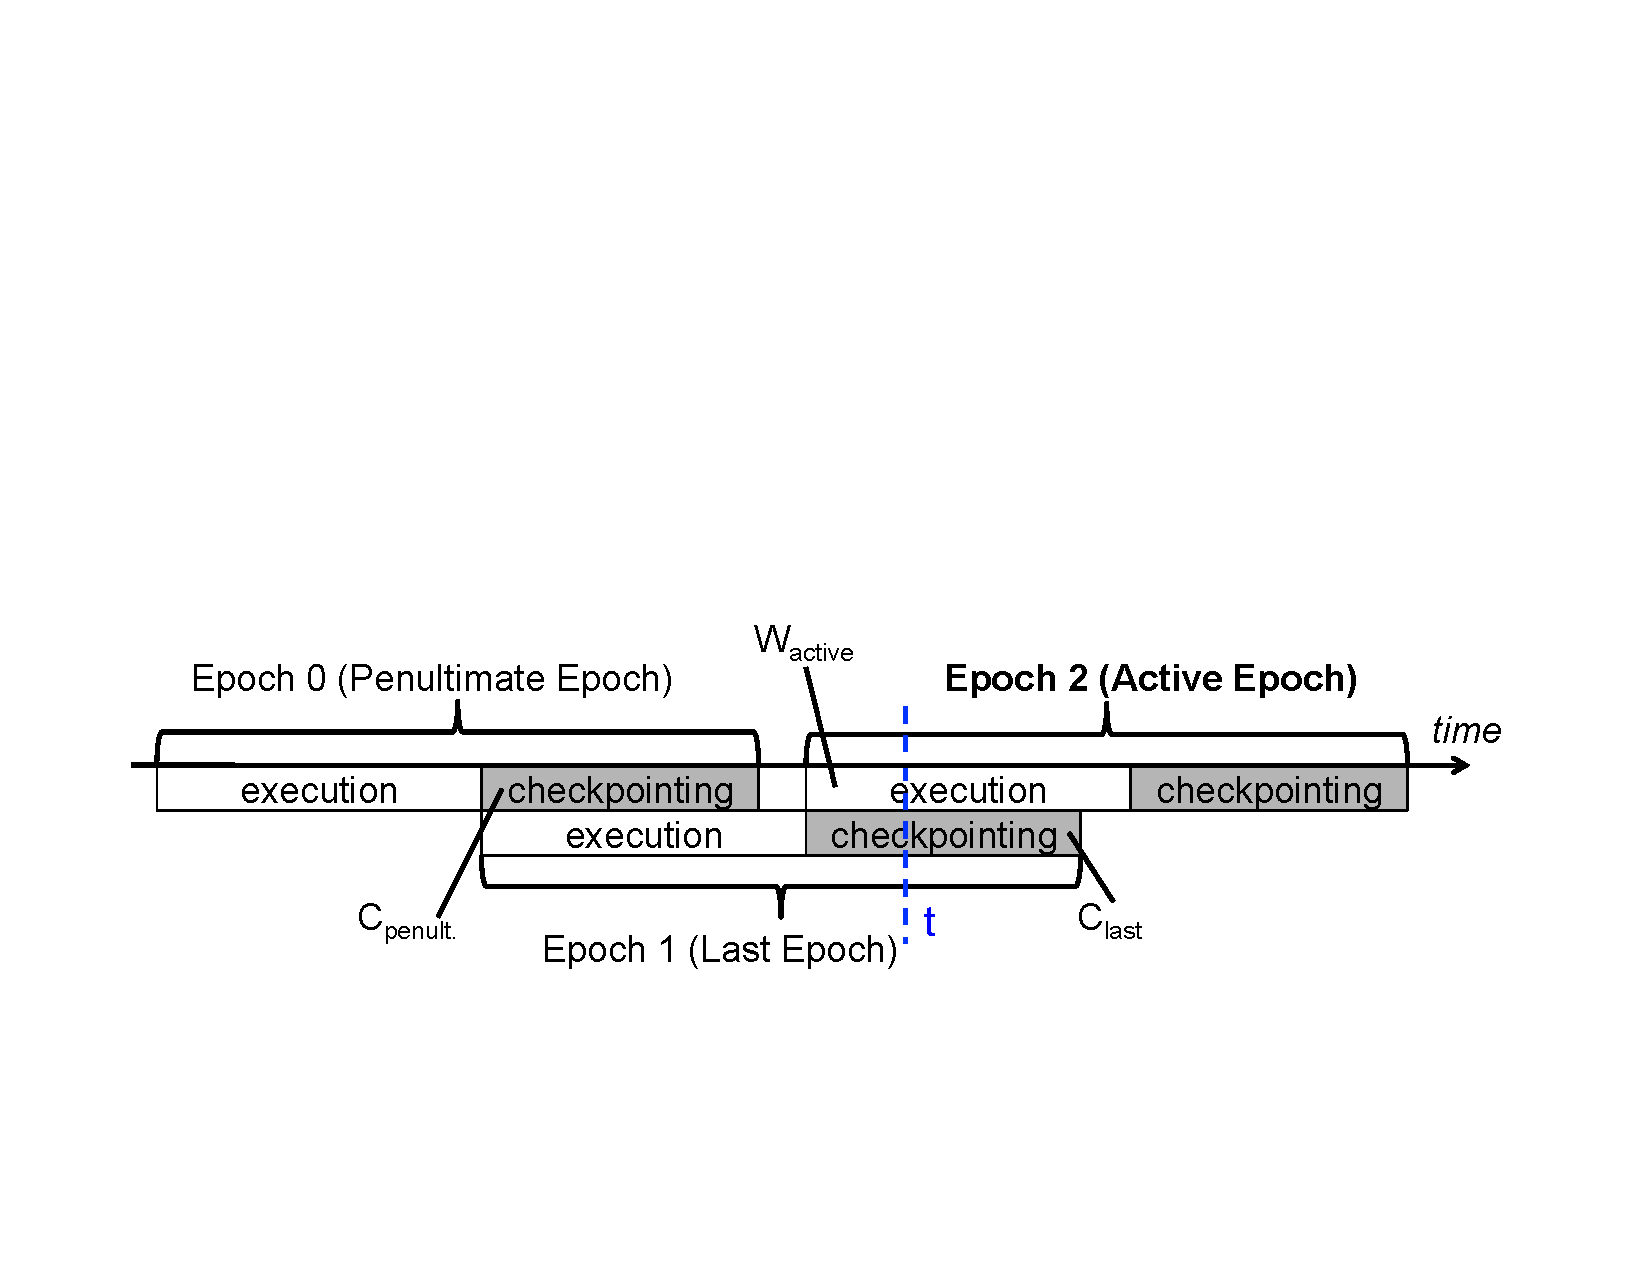
\includegraphics[width=0.9\columnwidth]{epoch-after}\\
{\small (b) THNVM采用的时间单元模型,可将检查点生成和程序执行相互重叠。该模型维护三个版本的数据:活跃的工作数据($W_{active}$)、最近检查点数据($C_{last}$),和次近检查点数据($C_{penult}$)。\hfill}
\caption{检查点生成系统的时间单元模型}
\label{fig-epoch}
\end{figure}

\textbf{时间单元模型}:我们逻辑上把程序的执行时间分成连续的时间区段,称为时间单元(epoch,如图\ref{fig-epoch})。每个时间单元包括一个执行阶段和一个检查点生成阶段。执行阶段更新工作数据,而检查点生成阶段持久化内存中的数据和CPU状态。

让执行阶段和检查点生成阶段顺次交替(如图\ref{fig-epoch}(a)所示)会导致显著的性能下降。对于内存访问频繁的负载,检查点生成可以消耗高达35.4\%的程序运行时间。所以,THNVM采用了一种将检查点生成阶段和程序执行阶段重叠的时间单元模型~\cite{1003568},以降低该性能损失。我们定义三个连续的时间单元依次为活跃的、最近的和次近的时间单元。如图\ref{fig-epoch}(b)所示,一个新的活跃时间单元(时间单元2)可以在最近时间单元(时间单元1)的执行阶段和次近时间单元(时间单元0)的检查点生成阶段两者中更晚结束的一个之后即开始。

\textbf{数据版本}:执行阶段和检查点生成阶段重合允许两个相邻的时间单元同时访问相同的数据。这对数据一致性的维护带来了两个挑战。第一,相互重合的执行阶段和检查点生成阶段可能会覆盖对方的数据更改,所以我们需要隔离不同时间单元的数据更改;第二,系统失效发生时,活跃时间单元和最近时间单元的数据可能被同时损坏。为了应对这些挑战,THNVM维护了连续时间单元下数据的三个版本:\emph{活跃的工作副本 $W_{active}$}、\emph{最近检查点$C_{last}$}和\emph{次近检查点$C_{penult}$} ($C_{last}$和$C_{penult}$既包括内存数据也包括CPU状态)。如图\ref{fig-epoch}(b)所示,当我们在执行时间单元2(更新$W_{active}$)的时候,THNVM会同时保留时间单元0的检查点($C_{penult}$)和时间单元1的检查点($C_{last}$);THNVM只有在时间单元1的生成检查点阶段结束后,才丢弃时间单元0产生的检查点。一个发生在时间$t$的系统故障,可能损坏时间单元2的工作数据副本以及时间单元1的检查点;此种状况下,我们可以依靠$C_{penult}$回滚到时间单元0。

\subsection{基于块重映射的检查点生成}
\label{subsec:block-remap}

THNVM对空间局部性低的数据更新使用块重映射模式进行管理。在每个时间单元的执行阶段,块重映射模式直接将工作数据写入NVM。因此,在相应的检查点生成阶段,THNVM可以简单地通过生成元数据(即BTT中的项)的检查点,将工作数据直接转为检查点数据。这样的方法可以大幅减少检查点生成的延迟。

为防止NVM中的更新损坏先前版本的数据,THNVM将新的缓存块的更改映射到一个其他的地址。THNVM将这类从原始地址到新地址的映射记录在BTT中。随后的内存读操作可以通过查找BTT来确定工作数据副本的有效位置。随后的以原始地址为目标的写操作,只要在同一个活跃时间单元内,可以进行归并,更新到该新地址。在下一个时间单元,该新地址的数据版本自然变为最近的检查点的一部分。NVM保存所有这些检查点数据;并且,THNVM在生成检查点阶段的开始会将BTT持久化到NVM。

\subsection{基于页回写的检查点生成}
\label{subsec:page-writeback}

页回写模式用于在页粒度上生成空间局部性较高的写操作的检查点。THNVM使用DRAM作为工作数据副本的缓冲。它首先在DRAM上归并内存的更新,然后在每个时间单元结束时生成检查点,将所有DRAM的脏页回写到NVM上。

这里的DRAM在两方面不同于CPU回写缓存或者简单的数据缓冲。第一,内存访问不会触发任何页置换或剔除;脏页只有在生成检查点时被回写。第二,当THNVM从DRAM回写一个脏页到NVM时,不可以直接覆盖NVM上原有的检查点数据。所以THNVM需要将每个脏页重定向到一个不同的地址上。THNVM使用PTT来为内存中的数据页追踪这些地址映射。在检查点生成结束的时候,PTT会被自动持久化到NVM上。这个标志着一个时间单元的结束。

\subsection{双重检查点生成机制}
\label{subsec:coordination}

\section{一致性机制的状态机表达}

\section{一致性机制的正确性证明}

\section{系统实现}

\subsection{地址空间管理}

\subsection{元数据管理}

\subsection{数据保存}

\subsection{数据恢复}

\section{系统测评}

\subsection{实验设置}

\subsection{微基准测试}

\subsection{存储类基准测试}

\subsection{计算类基准测试}

\subsection{敏感度分析}

\section{本章小结}

